% Drawing 154/04-6 -- folder 154, batch 04, archive page 73 (PDF page 74).
% Transcription: figures en tête de la page : un réseau de hachures vert foncé et jaune coupé par deux pseudo-droites rouges qui se croisent sur une droite pointillée, un petit segment épais noir au croisement ; légendes $\omega_{D'}$, $\omega_D$ (flèches), $\omega_F$ et $\omega_{F'}$ (flèches courbes). Une accolade renvoie à une seconde figure analogue, légendée « ou $(a', b')$ » et, à droite, « \uncertain{Cas} un peu vicieux, et sans intérêt ! »
% Kind: hatched net cut by two crossing pseudolines; a second analogous figure. Method 2 (schematic redraw from the facsimile). Status: partial.
% Notes: Head of the page: a net of dark green and yellow hatching cut by two red pseudolines crossing on a dotted line, a short thick black segment at the crossing; legends omega_{D'}, omega_D (arrows), omega_F and omega_{F'} (curved arrows, drawn as labels). A brace sends to a second analogous figure, legend « ou (a', b') »; the sentence « Cas un peu vicieux, et sans intérêt ! » to the right is text of the transcription. Read from the page view: the hatching is regularised (his strokes are uneven in spacing and colour). Still differs from the facsimile: the dark green and yellow hatchings are regularised (evenly spaced strokes), not traced stroke by stroke, in both figures.
% Coordinates: 1 unit = 1 mm = 1/100 of the crop width (bbox in page fractions: [0.116, 0.092, 0.628, 0.214]).
% Redrawn by Claude (claude-opus-5-5), issue #73, 2026-11-07; not checked by a human; not compiled (no TeX in the session).
% Revised by Claude (claude-opus-5-5) 2026-11-09 (issue #128) after Michel's check: vertices snapped to exact intersections (drawn points on their lines, meeting ends on the stroke they meet, near-concurrent lines through one computed point, curve ends on their rim); labels at \small as in folder 80 batch 3. Status: partial.
% Rights: reproduces part of the work -- behind RENDER_TRANSCRIPTS, never published by itself.
\documentclass[tikz,border=3pt]{standalone}
\usepackage{amsmath,amssymb}
\usetikzlibrary{patterns,arrows.meta}
\tikzset{Or/.style={orange!90!black}, Ye/.style={yellow!80!orange}, Lg/.style={green!60!black!70}, Dg/.style={green!45!black}, Br/.style={brown!80!black}, Rd/.style={red!85!black}, Bl/.style={blue!70!black}, Gy/.style={black!40}, pencil/.style={black!45}, struck/.style={black!35}, mark/.style={circle,draw,inner sep=1.3pt}, pt/.style={circle,fill,inner sep=0.9pt}, opt/.style={circle,draw,fill=white,inner sep=1.1pt}}
\begin{document}
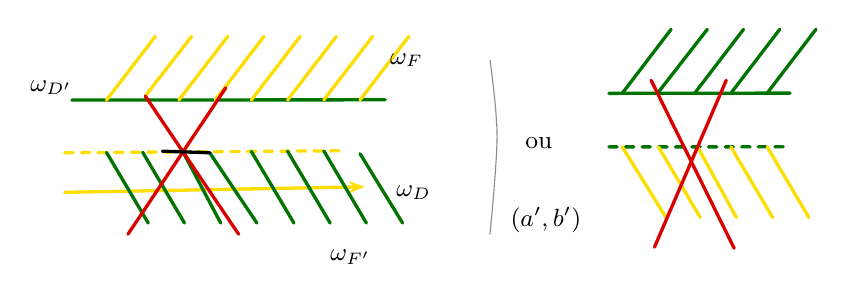
\begin{tikzpicture}[x=1mm,y=1mm,line cap=round,line join=round,font=\scriptsize]
\draw[Dg,very thick] (5.3,-11.28) -- (45.1,-11.25);
\draw[Ye,dashed,very thick] (4.41,-17.97) -- (39.82,-17.72);
\draw[Ye,very thick,-{Stealth[length=2mm]}] (4.4,-23) -- (42.5,-22.3);
\draw[Ye,very thick] (9.7,-11.28) -- (15.9,-3.2);
\draw[Dg,very thick] (9.7,-17.93) -- (15,-26.9);
\draw[Ye,very thick] (14.62,-10.77) -- (20.5,-3.2);
\draw[Dg,very thick] (14.29,-17.9) -- (19.6,-26.9);
\draw[Ye,very thick] (18.9,-11.27) -- (25.1,-3.2);
\draw[Dg,very thick] (19.41,-17.86) -- (24.2,-26.9);
\draw[Ye,very thick] (23.5,-11.27) -- (29.7,-3.2);
\draw[Dg,very thick] (22.8,-17.97) -- (28.8,-26.9);
\draw[Ye,very thick] (28.1,-11.27) -- (34.3,-3.2);
\draw[Dg,very thick] (28.09,-17.8) -- (33.5,-26.9);
\draw[Ye,very thick] (32.7,-11.26) -- (38.9,-3.2);
\draw[Dg,very thick] (32.69,-17.77) -- (38.1,-26.9);
\draw[Ye,very thick] (37.3,-11.26) -- (43.5,-3.2);
\draw[Dg,very thick] (37.3,-17.74) -- (42.7,-26.9);
\draw[Ye,very thick] (41.9,-11.26) -- (48.1,-3.2);
\draw[Dg,very thick] (41.9,-18.1) -- (47.3,-26.9);
\draw[Rd,very thick] (14.62,-10.77) -- (26.48,-28.32);
\draw[Rd,very thick] (24.84,-9.73) -- (12.43,-28.32);
\draw[very thick] (16.8,-17.78) -- (22.8,-17.97);
\node[inner sep=1pt] at (2.7,-9.7) {\small $\omega_{D'}$};
\node[inner sep=1pt] at (48.7,-23) {\small $\omega_D$};
\node[inner sep=1pt] at (47.8,-6.2) {\small $\omega_F$};
\node[inner sep=1pt] at (40.7,-31.2) {\small $\omega_{F'}$};
\draw[pencil] plot[smooth, tension=0.55] coordinates {(58.4,-6.2) (59.3,-15.9) (58.4,-28.3)};
\node[inner sep=1pt] at (64.6,-16.8) {\small ou};
\node[inner sep=1pt] at (65.5,-26.5) {\small $(a',b')$};
\draw[Dg,very thick] (73.5,-10.43) -- (96.5,-10.4);
\draw[Dg,dashed,very thick] (73.5,-17.23) -- (96.5,-17.22);
\draw[Dg,very thick] (75.2,-10.42) -- (81.4,-2.3);
\draw[Ye,very thick] (75.2,-17.23) -- (80.85,-26.35);
\draw[Dg,very thick] (79.68,-10.42) -- (86,-2.3);
\draw[Ye,very thick] (79.8,-17.23) -- (85.1,-26.2);
\draw[Dg,very thick] (84.4,-10.41) -- (90.6,-2.3);
\draw[Ye,very thick] (84.77,-17.23) -- (89.7,-26.2);
\draw[Dg,very thick] (89,-10.41) -- (95.2,-2.3);
\draw[Ye,very thick] (89,-17.23) -- (94.3,-26.2);
\draw[Dg,very thick] (93.6,-10.4) -- (99.8,-2.3);
\draw[Ye,very thick] (93.6,-17.22) -- (98.9,-26.2);
\draw[Rd,very thick] (78.86,-8.77) -- (89.41,-30.1);
\draw[Rd,very thick] (88.41,-8.76) -- (79.29,-29.97);
\end{tikzpicture}
\end{document}
